\documentclass[nopreprintline,12pt]{elsarticle}
%\setcounter{secnumdepth}{1} %auf 0, wenn Sections nicht nummeriert werden sollen

\usepackage{fancyhdr}


\pagestyle{fancy}
\fancyhf{}
%\renewcommand{\sectionmark}[1]{ \markright{#1} }
\thispagestyle{empty}
\fancyhead[R]{\rightmark}
\fancyhead[L]{}
\fancyfoot[C]{\thepage}

\usepackage{todonotes} %für Markierungen
%\usepackage[disable]{todonotes} um alle gleichzeitig wegzukriegen

\fancypagestyle{frontmatter}   % für seiten mit chapter titel
{
  \fancyhf{}
  \fancyhead[R]{\rightmark}
  %\fancyhead[L]{\leftmark}
  %\lhead{}
  %\rhead{\leftmark}
  \fancyfoot[C]{\thepage}
}

\fancypagestyle{mainmatter}   % für seiten mit chapter titel
{
  \fancyhf{}
  \fancyhead[R]{\rightmark}
  %\fancyhead[L]{\leftmark}
  %\lhead{}
  %\rhead{\leftmark}
  \fancyfoot[C]{\thepage}
}

\renewcommand{\headrulewidth}{0.5pt}

\renewcommand{\chaptermark}[1]{%
\markboth{\thechapter. \ #1}{}}

\usepackage{newtxtext,newtxmath}

\usepackage{lipsum,graphicx,float}
\usepackage{caption}
%\usepackage{subcaption}
\usepackage{subfig}
%\usepackage{float}

\usepackage{amssymb}

\usepackage{lineno}

\usepackage{xcolor} %Text in Farbe

\usepackage[ngerman]{babel} %Deutsch
\usepackage[utf8]{inputenc}

\usepackage[onehalfspacing]{setspace} %Zeilenabstand

\usepackage[toc,page]{appendix}

%\makeatletter
%\def\ps@pprintTitle{%
%   \let\@oddhead\@empty
%   \let\@evenhead\@empty
%   \let\@oddfoot\@empty
%   \let\@evenfoot\@oddfoot
%}
%\makeatother

\setlength{\headheight}{15pt}


%% `Elsevier LaTeX' style
\usepackage{natbib}
\usepackage{apalike}
\bibliographystyle{apalike}
%%%%%%%%%%%%%%%%%%%%%%%
\author{Cristina Ballero Reque}
\title{Einfluss von Schlaf auf die Gedächtnisleistung}
\address{Ruhr-Universität Bochum}
\address{Arbeitseinheit Neuropsychologie}
\journal{Dr. Lorena Deuker}

\begin{document}

%\maketitle
%\pagenumbering{gobble}
%% Title, authors and addresses

\begin{frontmatter}
\begin{abstract}
    xkml
\end{abstract}
\begin{keyword}
Science \sep Publication \sep Complicated
\end{keyword}
\end{frontmatter}


%%%%%%%%%%%%%%%%%%%%%%%
%% Elsevier bibliography styles
%%%%%%%%%%%%%%%%%%%%%%%
%% To change the style, put a % in front of the second line of the current style and
%% remove the % from the second line of the style you would like to use.
%%%%%%%%%%%%%%%%%%%%%%%


%% APA style
%\bibliographystyle{model5-names}\biboptions{authoryear}

\newpage

\pagenumbering{gobble}

\newpage

\todo[inline]{Einleitung}
\todo[inline]{anderer Titel!}
\todo[inline]{Abstract}
\todo[inline]{Graphenstruktur-Graphik einfügen (2.3)}
\todo[inline]{Hintergrund für Statistik-Entscheidungen? --> Eid/LEA}
\todo[inline]{Diskussion: Referenzen für Integration in blabla}
\todo[inline]{Diskussion: Implikationen}
\todo[inline]{Diskusison: Ausblick}
\todo[inline]{Wie zitiert man Anhang und Abb./Tabellen? --> Kim?}
\todo[inline]{Fragebögen und LANDSCHAFTSBILDER in den Anhang packen!}
\todo[inline]{Fußnoten aus Titlepage raus --> oddempty?}

\pagenumbering{gobble}
\tableofcontents
\clearpage
\pagenumbering{arabic}
\newpage

\pagestyle{mainmatter}
\section{Einleitung}
\label{S:1}
\paragraph{Blabla toller Aufhänger}
%Wir alle sind umgeben von Gemeinschaften, wie z.B. die Familie, Nachbarschaft, Studierendenschaft etc.. Es gibt jedoch noch viel mehr Gemeinschaften, als und bewusst sind. Auch zeitlich können Objekte als zusammengehörig gruppiert werden, meist implizit.
%Das erlernen wir ein ganzes Leben lang, ohne uns darüber bewusst zu werden, wie wir Dinge kategorisieren (Studien 8-10 aus Shapiro_2013). Neue Idee von \citet{Shapiro_2013}: auch temporale Zusammenhänge können erlernt werden.
%Hier noch Bezug zur Garvert-Studie zu nicht-räumlichem Lernen.

%--> Event-Segmentation-Theorie von Radvansky?

\textcolor{blue}{Hier noch coolen Alltagsbezug finden!}
Nach \cite{Kurby2008} nehmen wir die Welt nicht als ununterbrochenen Strom wahr, sondern unterteilen sie in koherente Ereignisse, die wiederum aus einzelnen Sequenzen bestehen. Die Event-Segmentation-Theorie von \cite{Zacks2007} besagt, dass diese Einteilung erfolgt, um kommende Information zu antizipieren.
Was dabei zusammengehört und was nicht, kategorisieren wir für semantische Inhalte nach \cite{Medin1978} aufgrund von geteilten Attributen wie z.B. Form, Verhalten und Funktion. Ereignisse können auf ähnliche Art eingeordnet werden: aufgrund ihrer zeitlichen Nähe zueinander \citep{Schapiro2013}. Die Zuordnung und Unterteilung von Ereignissen erfolgt dabei automatisch und ohne, dass wir uns darüber bewusst sind \citep{Kurby2008}, es findet also implizites Lernen statt. \cite{Berry1993} beschreibt implizites Lernen als den unbeabsichtigten Erwerb neuer Informationen, die später nur schwer verbalisierbar sind und sich intuitiv im Verhalten wiederspiegeln \citep{Kamiya2015}.

\paragraph{Organisation im Gehirn}
Damit wir (implizit) neu Erlerntes später abrufen können, müssen die Informationen und Assoziationen in einer Struktur organisiert werden \citep{Garvert2017}.
Die Organisation von zeitgleich auftretenden Stimuli wird dabei durch den Hippocampus unterstützt \citep{Schapiro2013}.
Sowohl im Hippocampus als auch im angrenzenden entorhinalen Cortex werden Assoziationen und Beziehungen zwischen Objekten, sowie deren Position im Raum reflektiert \citep{Horner2015, Schapiro2013}.
Wie \cite{Garvert2017} zeigen konnten, werden dazu unbewusst mentale Karten angelegt. In ihnen werden räumliche und abstraktere, nicht-räumliche Beziehungen wie z.B. die von Ereignissen, sich sich oft zeitlich nah ereignen, abgebildet.
Diese mentale Repräsentation von Zusammenhängen hilft den Autoren zufolge dabei, unser Verhalten zu lenken und aus bereits Gelerntem Interferenzen zu ziehen.

\paragraph{Gedächtnissysteme}
Von impliziten bzw. nicht-deklarativen Gedächtnisinhalten und ihrem Erwerb ist das explizite bzw. deklarative Gedächtnis abzugrenzen \citep{Squire1996}, dessen Inhalte bewusst reproduziert werden können. Die vorliegende Studie befasst sich mit dem Erlernen impliziter Strukturen, für deren Erwerb und Abruf weniger Aufmerksamkeit benötigt wird \citep[see][]{Gruber}.

%Dadurch, dass der Erwerb und der Abruf hierbei implizit und automatisch erfolgt, werden weniger Aufmerksamkeitsressourcen als beim Erwerb und Abruf von deklarativen Gedächtnisinhalten benötigt (Gruber, 2018)

%%%%%%%%%%%% VON JU %%%%%%%%%%%%%%%
%Erstaunlicherweise verbringt der Mensch ungefähr ein Drittel seines gesamten Lebens im Zustand des Schlafes (Terrence \& Destexhe, 2000). Es gibt viele verschiedene Funktionen des Schlafes, wovon eine sehr wahrscheinlich die Konsolidierung von neuen Gedächtnisinhalten darstellt. 
%Die Konsolidierung bezeichnet den Vorgang, indem zunächst instabile Gedächtnisspuren, in stabilere verfestigt werden (Diekelmann \& Born, 2010). Dadurch können neu enkodierte Informationen in das Langzeitgedächtnis überführt werden (Diekelmann \& Born, 2010). 

%Verschiedene Untersuchungen konnten hier einen positiven Einfluss von Schlaf auf die Konsolidierung von deklarativen, also bewussten sowie nicht-deklarativen, also unbewussten Gedächtnisinhalten nachweisen (Chambers, 2017; Rasch \& Born, 2013; Born, Rasch, \& Gais, 2006). 
%Es bleibt jedoch noch ungeklärt, ob sich ein Schlafzyklus auch positiv auf die Konsolidierung des impliziten Erwerbs von neuen deklarativen Gedächtnisinhalten und somit auch positiv auf die Erinnerungsleistung auswirkt. Daher ist das Ziel der vorliegenden Arbeit, einen möglichen moderierenden Einfluss von Schlaf auf die Interaktion zwischen diesen beiden Gedächtnissystemen zu belegen.


\paragraph{Implizites Lernen}
%Mentale Repräsentationen werden oft implizit erworben/erlernt (Hier Studie von Seger_1994?).
%Dann Hirnstrukturen zum Erwerb von implizitem Lernen (oder Unterscheidung von deklarativ vs. nicht-deklarativ). Implizit Gelerntes zeigt sich auch im Verhalten.
%Gedächtnisbildung 3 Phasen: neue Ereignisse/Wissensinhalte müssen enkodiert und konsolidiert werden, damit sie später (korrekt) abgerufen werden können. Dafür zwei Hirnstrukturen wichtig (Garvert_2017), die auch wichtig sind für Inferenz-Denken.



%\paragraph{Unterteilung KZG/LZG}
%Grundlagentext moodle
%Deklarativ/nicht deklarativ


\paragraph{Gedächtnis(konsolidierung) und Schlaf}
%Bedeutung von Schlaf für die Konsolidierung in den letzten Jahren/Jahrzehnten immer mehr erforscht und bestätigt.
Review Rasch \& Born
--> Unterteilung in Schlaf-/Taggruppe
Vorteile von Schlaf auf (wenn möglich) implizites (prozedural) Lernen

evtl. Studie zu Mittagsschlaf (sonst in Diskussion als post-hoc)


\section{Methoden}
\label{S:2}

\subsection{Stichprobe}
Die Erhebung erstreckte sich über einen vierwöchigen Zeitraum von Ende April bis Mitte Mai 2018. Dabei nahmen insgesamt 52 Versuchspersonen an der Studie teil. Aufgrund einer Änderung der  EU-weiten Datenschutzrichtlinien wurden keine soziodemographischen Daten erhoben. Voraussetzung für die Teilnahme an der Studie waren ein Mindestalter von 18 Jahren, eine ausreichende (evtl. korrigierte) Sehkraft. Um Beeinträchtigungen der Erinnerungsleistung zu minimieren, wurden die ProbandInnen außerdem angewiesen, unmittelbar vor der Testung sowie in den darauffolgenden zwölf Stunden keinen Alkohol zu konsumieren. Außerdem wurden Personen ausgeschlossen, die an Epilepsie erkrankt sind.
Die Studie wurde im Rahmen eines universitären Seminars durchgeführt, bei dem mehrere Studierende zusammenarbeiteten. Die Rekrutierung der Studienteilnehmer wurde daher auf die Beteiligten aufgeteilt. Jeder Studierende sollte nach Möglichkeit vier Personen in seinem privaten Umfeld für die Studie anwerben und testen. Es gab keine Vergütung für die Teilnahme an der Studie.

\subsection{Versuchsdesign}
Zur Überprüfung der Hypothesen und zur Vermeidung von Lern-Effekten wurde ein Between-Subject Versuchsdesign gewählt. Dazu wurden die ProbandInnen im Vorhinein zufällig einer von zwei Gruppen zugeteilt, die als „Schlafgruppe“ (n = 25) und „Taggruppe“ (n = 27) benannt wurden. Die beiden Gruppen unterschieden sich hinsichtlich der Zeitpunkte, zu denen die zweiteilige Studie durchgeführt wurde. ProbandInnen der Schlafgruppe führten den ersten Teil abends durch und absolvierten den folgenden Teil am darauffolgenden Morgen. Bei der Taggruppe fand die Testung im Laufe eines Tages statt; morgens wurde der erste, abends der zweite Teil bearbeitet. Wichtig dabei war die Einhaltung eines zwölfstündigen Zeitraums zwischen beiden Testungen.

\subsection{Versuchsaufbau}
Die Studie wurde mittels des Simulationsprogramms \textit{Matlab\_R2018a} an den Computern der Studierenden durchgeführt. Die verwendeten Stimuli waren im Vorhinein von der Arbeitseinheit für Neuropsychologie in einem 3D-Programm  erstellt worden. Es \textcolor{purple}{handelt} sich dabei um fiktive Objekte in Grautönen, die möglichst keine Ähnlichkeit zu Alltagsgegenständen haben sollten. Dies wurde mittels eines Fragebogens abgesichert, den die Seminarteilnehmenden vor Beginn der eigentlichen Testung ausfüllten. Die angegebenen Assoziationen der Stimuli zu Alltagsgegenständen führten zum Ausschluss von zweien der ursprünglich 20 Stimuli. Von jedem Stimulus gab es eine Standardversion \textit{(a)} und eine Version in rotierter Ausrichtung \textit{(b)} (Vgl. Abb. 1). Letztere wurde von einem Teil der Studierenden erstellt und nahm später die Funktion eines Distraktors ein.

\begin{figure}[h]
%\begin{subfigure}{0.5\textwidth}
\centering
\setkeys{Gin}{width=4.5in,height=4.5cm,keepaspectratio}%
\subfloat[Original]{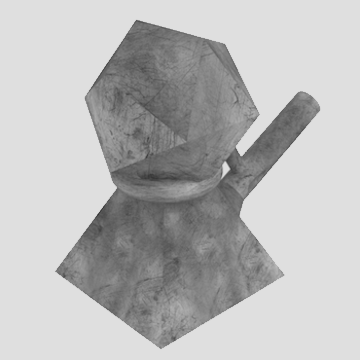
\includegraphics{Bilder/Objekt11A.png}}
\hspace{1cm}
\subfloat[Rotiert]{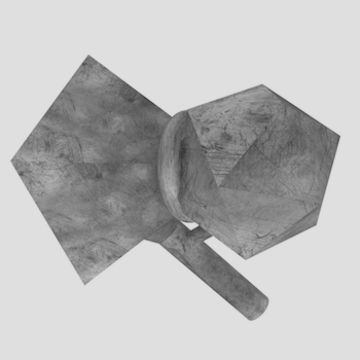
\includegraphics{Bilder/Objekt11B.png}}
%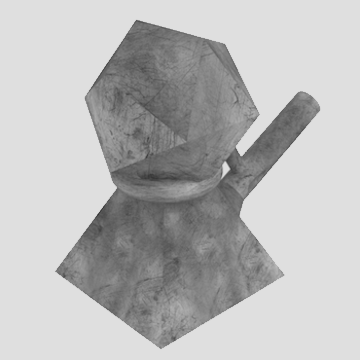
\includegraphics[width=0.9\linewidth, height=5cm]{Bilder/Objekt11A.png}
%\caption{Original}
\label{fig:subim1}
%\end{subfigure}
%\begin{subfigure}{0.5\textwidth}
%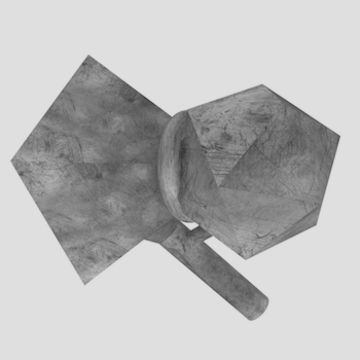
\includegraphics[width=0.9\linewidth, height=5cm]{Bilder/Objekt11B.png}
%\caption{Rotiert}
\label{fig:subim2}
%\end{subfigure}
\caption{Beispielhafter Stimulus in zwei Ausrichtungen}
%\label{fig:image2}
\end{figure}

Aus den verbliebenen 18 Stimuli wurden drei gleich große Gruppen gebildet, die als \textit{Communities} bezeichnet wurden. Dabei war die Zuordnung von jeweils sechs Stimuli zu einer Community für jede Versuchsperson randomisiert.
Diese Anordnung der Stimuli geschah in Anlehnung an die Studie von \citet{Schapiro2013} in Form einer Graphenstruktur. Jeder Stimulus  hat dabei eine direkte Verbindung zu drei weiteren Stimuli. Damit sind Mitglieder einer Community häufiger miteinander verbunden also mit anderen. Am Rand jeder Community gibt es jeweils einen Stimulus, Grenz-Stimulus genannt, dessen dritte Verbindung zum Grenz-Stimulus der nächsten Community reicht.
\todo[inline]{HIER ein Bild der GRAPHENSTRUKTUR einbauen!}


\subsection{Versuchsablauf}
Das Experiment war in zwei Teile unterteilt, die von allen Studienteilnehmenden in gleicher Reihenfolge absolviert wurden.

\paragraph{Encoding} Im ersten Teil, dem \textit{Encoding} sollten die ProbandInnen mit den Stimuli vertraut gemacht werden. Dazu wurden Sequenzen der Stimuli mit einer Target-Detektions-Aufgabe verbunden. Die Reihenfolge entstand dabei durch einen sog. \textit{Random Walk} über die oben beschriebene Graphenstrultur.
Zu Beginn gab es nach einer Instruktion durch die Versuchsdurchführenden 20 Trials zur Übung, bei denen vor einem weißen Hintergrund \textcolor{purple}{in 5\% der Fälle} ein Distraktor (ein graues Rechteck) erschien, der mittels Tastendruck detektiert werden sollte. \textcolor{purple}{Zu langer Satz?}

Daraufhin begann die eigentliche Aufgabe mit insgesamt 720 Trials, die in sechs gleich großen Blöcken (à 120 Trials) gezeigt wurden. Bei den ersten drei Durchgängen sollten die Versuchsteilnehmenden den Distraktor wie zuvor in Form eines grauen Rechtecks \textcolor{purple}{(redundant?)} identifizieren. In den folgenden Durchgängen fungierten, wie bei \citet{Schapiro2013}, die Objekte in rotierter Version als Distraktor. Die Häufigkeit, mit der die zu identifizierenden Targets erschienen, war zuvor von den Versuchsdurchführenden festgelegt worden: das graue Kästchen tauchte in 5\% der Fälle auf, die rotierten Objekte in 15\%. Durch die geringe Auftretenswahrscheinlichkeit sollte eine stabil hohe Konzentration der ProbandInnen gewährleistet werden. Diese wurde als Voraussetzung zum impliziten Erlernen der Graphenstruktur gesehen.
Während der Trials wurden die Stimuli jeweils für eine Sekunde dargeboten, wonach sie verblassten und nach ebenfalls einer Sekunde der nächste Stimulus auftauchte. Zwischen jedem Block gab es eine Pause, in der neun Landschaftsbilder für jeweils zehn Sekunden dargeboten wurden. Die Landschaftsbilder wurden bei der Versuchsplanung von der Seminarleitung ausgewählt und sollten der Entspannung zwischen den einzelnen Durchgängen dienen. Außerdem wurde nach dem dritten Block (am Ende der Pause) der Wechsel des Distraktorentyps angekündigt. Insgesamt betrug damit die Dauer des ersten Teils etwa 35 Minuten.

\paragraph{Retrieval} Der zweite Teil der Studie, das \textit{Retrieval} war in zwei verschiedene Aufgaben unterteilt, die im Vergleich zum Encoding-Teil eine kürzere Bearbeitungszeit hatten. Daher wurden die Instruktionen für beide Aufgaben gleichzeitig gegeben.

Bei der ersten Aufgabe des Retrievals, \textit{Odd-one-out}, wurden zu Beginn in acht Übungsdurchgängen jeweils drei Landschaftsbilder nebeneinander angeordnet gezeigt. Unter den drei Bildern sollten die ProbandInnen diejenige Landschaft auswählen, die ihrem subjektiven, intuitiven Eindruck nach nicht dazugehört. Dazu konnte innerhalb eines bestimmten Zeitfensters (2.5 s) eine von drei Tasten gedrückt werden, die jeweils einer Position der Bilder entsprach (links, mittig, rechts). Ein Pausieren während dieser siebenminütigen Aufgabe war nicht möglich. Bei einer Reaktion außerhalb des vorgegebenen Zeitfensters erschien ein Hinweis auf dem Display mit der Bitte um schnellere Antwort. Nachdem die Teilnehmenden die Zuordnung der Tasten gelernt und sich an das Antwortzeitlimit gewöhnt hatten, wurden anstelle der Landschaftsbilder die eigentlichen Stimuli angezeigt. Die drei angezeigten Stimuli, auch \textit{Triplet} genannt, stammten aus verschiedenen Kategorien. Sie unterschieden sich bezüglich ihrer Distanz und Community-Zuordnung auf der zugrundeliegenden Graphenstruktur. Vor Versuchsbeginn waren acht verschiedene Kategorien identifiziert worden, aus denen jeweils maximal 18 Triplets präsentiert werden sollten. Welcher Stimulus dabei an welcher Position präsentiert wurde, wurde randomisiert. Zusätzlich wurden für die spätere Auswertung im Vorhinein pro Kategorie diejenigen Stimuli identifiziert, die aufgrund der Graphenstruktur (nicht) ausgewählt werden sollten.

Aufgabe der zweiten Retrieval-Aufgabe, \textit{Sorting}, war es, die Stimuli zu sortieren. Ohne eine konkrete Zeitvorgabe sollten die Teilnehmenden dabei die kreisförmig angeordneten Objekte durch drag and drop anordnen. Für die Einteilung wurden wie bei der vorigen Aufgabe keine konkreten Kriterien gegeben; die ProbandInnen sollten auch dann eine Entscheidung treffen, wenn sie keine Regeln zu erkennen meinten. Die Positionierung wurde von den ProbandInnen selbst durch Tastendruck abgeschlossen, zuvor war es ihnen beliebig oft möglich, zur ursprünglichen Anordnung zurückzukehren. Wichtig für die spätere Auswertung war der Abstand der einzelnen Objekte zueinander entlang einer horizontalen und einer vertikalen Achse.

Abgeschlossen wurde der zweite Teil und damit die Studie durch einen kurzen Fragebogen, den die ProbandInnen ausfüllen sollten. Je nachdem, ob sie der Tag- oder Schlafgruppe zugeordnet worden waren, sollten sie ihren Tagesablauf beschreiben und bewerten bzw. Angaben zu Schlafzeiten und -qualität machen. Außerdem hatten alle Teilnehmenden die Möglichkeit anzugeben, ob ihnen bei der Durchführung des Experiments etwas aufgefallen sei.

\subsection{Statistische Analysen}
Für die Datenanalyse wurde das Open Source Statistikprogramm R (Version 3.5.0, \textit{R Studio}) verwendet.
Es wurde zwischen beiden Unteraufgaben des zweiten Teils der Studie (\textit{Retrieval}) unterschieden.

\paragraph{Odd-one-out}
Beim \textit{Odd-one-out} war vorab für die Kategorien 2,3,4,6 und 8 festgelegt worden, welcher Stimulus von den ProbandInnen aufgrund der Graphenstruktur aussortiert (gewählt) werden sollte, sofern diese erlernt wurde.Dafür wurde im Vorhinein eine Tabelle erstellt (s. Anhang). Am Beispiel der in Abbildung 2 dargestellten \textcolor{purple}{Triplet-Sequenz} soll für Kategorie 4 erläutert werden, welcher Stimulus von den ProbandInnen als weniger passend identifiziert werden sollte. Objekt A und B befinden sich in derselben Community und sind direkt miteinander verbunden. Auch zwischen den Objekten B und C besteht eine direkte Verbindung, C gehört jedoch einer anderen Community an. Wenn die Graphenstruktur erlernt wurde, sollte Objekt C als unpassend identifiziert und ausgewählt werden, da es zu einer Community außerhalb gehört.

\begin{figure}[h]
    \centering
    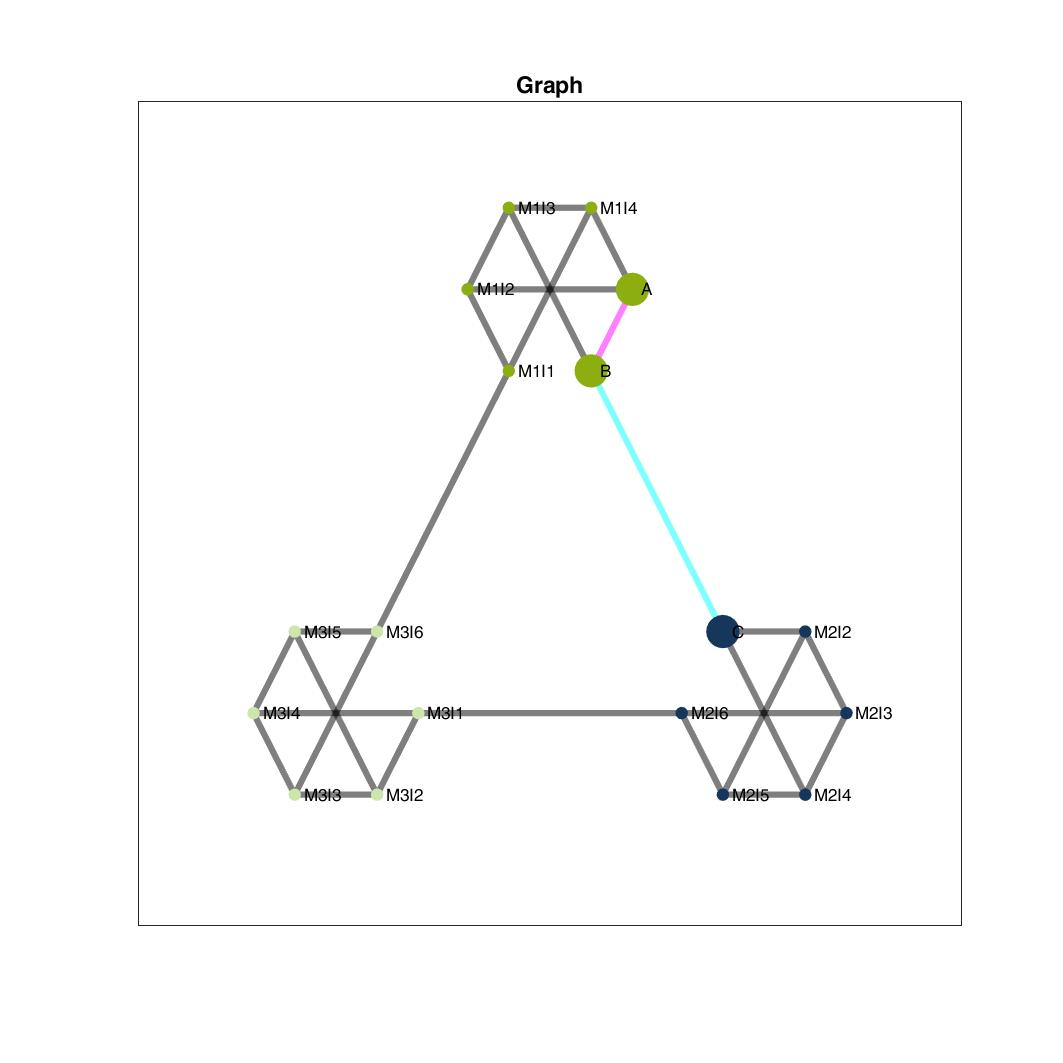
\includegraphics[width=85mm]{cat04_2716_tripletVisual.jpg}
    \caption{Beispielhafte Graphenstruktur für Kategorie 4}
    \label{fig:my_label}
\end{figure}
\todo[inline]{Leas Version der Graphik nehmen?}


Aus der Anzahl der richtig identifizierten Stimuli für diese Kategorien wurde eine Trefferquote errechnet. Anschließend wurde diese für alle Teilnehmenden gemittelt und mittels \textit{t}-Test mit der Ratewahrscheinlichkeit verglichen. Bei drei Auswahlmöglichkeiten kann davon ausgegangen werden, dass die Wahrscheinlichkeit, durch Raten den richtigen Stimulus zu identifizieren, 1/3 beträgt.
Für Kategorie 1 und 5 war nicht eindeutig, welcher Stimulus als nicht/weniger zugehörig auszuwählen war. In Kategorie 1 gehörten alle Stimuli derselben Community an, der mittlere Stimulus war mit den anderen beiden direkt verbunden. Die äußeren Stimuli waren miteinander nur über zwei Schritte verbunden, daher sollte einer von beiden ausgewählt werden, nicht aber der mittlere.
In Kategorie 5 waren zwei Stimuli aus derselben Community über drei Schritte miteinander verbunden. Einer von ihnen war außerdem mit dem dritten Stimulus aus einer anderen Community direkt verbunden. Dabei sollte Letzterer auf Basis der Graphenstruktur ausgewählt werden, bzw. nicht der mittlere Stimulus.
Kategorie 7 umfasste Stimuli aus drei verschiedenen Communities, die gleich weit voneinander entfernt waren, daher sollte dort zufällig ein Stimulus gewählt werden.
\textcolor{blue}{sollte ich die überhaupt alle beschreiben? Tabelle ist ja auch im Anhang..?}

\paragraph{Sorting}
Für den zweiten Teil des Retrievals wurde für jeden ProbandInnen die Distanz errechnet, die zwischen den von ihm/ihr angeordneten Stimuli lag.
Auch für den zweiten Teil des Retrievals fand die Auswertung zunächst für jeden einzelnen Teilnehmenden statt, danach wurde ein Gruppendurchschnitt errechnet. Zunächst wurde die Distanz zwischen den von den ProbandInnen angeordneten Stimuli untereinander berechnet. Daraufhin wurde die Zugehörigkeit jedes Stimulus zu seiner Community bestimmt. Dadurch konnte die durchschnittliche Distanz berechnet werden zwischen Objekten innerhalb einer Community und der Distanz zu Stimuli, die einer anderen Community zugewiesen worden waren. Abschließend wurde mit einem gepaarten \textit{t}-Test überprüft, ob sich die durchschnittliche Distanz innerhalb von der Distanz außerhalb einer Community signifikant unterscheidet. Dabei wurde zwischen der Tag- und der Schlafbedingung unterschieden.

\subsection{Spezifische Hypothesen}

\paragraph{Hypothese 1 – Implizites Lernen der Struktur}
Die erste Hypothese lautete, dass die ProbandInnen die implizite Community-Struktur lernen.
Die Hypothese sollte als bestätigt gewertet werden, wenn beim \textit{Odd-one-out} der (laut Tabelle) richtige Stimulus signifikant häufiger ausgewählt wurde als die anderen. Beim \textit{Sorting} sollten die Stimuli einer Community einen geringeren Abstand untereinander haben als zu Stimuli einer anderen Community.

\paragraph{Hypothese 2 – ProbandInnen zeigen Interferenz}
Laut Hypothese 2 sollten die ProbandInnen aus den nacheinander präsentierten Stimuli Schlüsse über die Beziehung von Stimuli ziehen können, die nicht direkt nacheinander gezeigt wurden. Objekte einer Community, die keine direkte Verbindung miteinander hatten, sollten also trotzdem als zueinander ähnlicher empfunden werden, als zu Objekten anderer Communities.
Daher sollten in Kategorie 3 und 5 des \textit{Odd-one-out} diejenigen Stimuli gewählt werden, die zwar eine direkte Verbindung zum mittleren Stimulus hatten, jedoch zu einer anderen Community gehörten.

\paragraph{Hypothese 3 – Einfluss von Schlaf}
Es wurde weiterhin davon ausgegangen, dass Schlaf einen positiven Einfluss auf die Konsolidierung der Graphenstruktur hat. Daher wurde hypothetisiert, dass ProbandInnen der Schlaf-Schlafbedingung bei beiden Teilen des \textit{Retrievals} signifikant bessere Ergebnisse erzielen als die der Taggruppe.

\section{Ergebnisse}
\label{S:3}
Bei der Datenauswertung wurden drei ProbandInnen ausgeschlossen. Grund dafür waren technische Probleme, Probleme mit dem Verständnis der zweiten Aufgabe sowie mangelnde Konzentration im ersten Teil.
Ein(e) weitere StudienteilnehmerIn wurde nicht in die statistische Analyse aufgenommen, da in der Sorting-Aufgabe lediglich ein Item bewegt wurde. Damit wurde die Aufgabe als nicht ausreichend bearbeitet angesehen.

Da die gesamte Stichprobe größer als n=30 war, konnte für die allgemeinen Analysen (ohne Unterscheidung der Bedingungen) von einer Normalverteilung und Varianzhomogenität der Ergebnisse ausgegangen werden. Damit waren die Voraussetzungen für einen \textit{t}-Test gegeben.

\subsection{Wichtigste Befunde}
\paragraph{Odd-one-out}
Die durchschnittliche Trefferquote im ersten Teil des Retrievals, \textit{Odd-one-out}, für die jeweiligen Kategorien ist in Tabelle 1 dargestellt. \textcolor{blue}{what about SD und Effektstärken?}. Für Kategorie sechs wurde über alle ProbandInnen gemittelt die höchste Trefferquote erzielt (\textit{M =} 36.2\%).
Der gerichtete \textit{t}-Test ergab, dass die Anzahl der richtig identifizierten Stimuli im Vergleich zur Ratewahrscheinlichkeit nicht signifikant höher war. Dies zeigte sich über alle analysierten Kategorien hinweg.

\begin{table}[h]
\centering
\begin{tabular}{l c c} %%l,c,r für Ausrichtung des Textes (links, mittig, rechts)
\hline
\textbf{Kategorie} & \textbf{Trefferquote} & \textbf{p-Wert}\\
\hline
2 & 32.1 & 0.723\\
3 & 33.5 & 0.471\\
4 & 33.6 & 0.433\\
6 & 36.2 & 0.163\\
8 & 33.6 & 0.436\\
\hline
\end{tabular}
\caption{Note. Trefferquote in Prozent}
\end{table}

Für Kategorien 1 und 5 wurde angenommen, dass der mittlere Stimulus weniger häufig ausgewählt werden sollte als die Ratewahrscheinlichkeit. Der gerichtete \textit{t}-Test wurde nicht signifikant für Kategorie 1 (\(\textit{T}_{[48]}\) = 0.51, \textit{p} = 0.69) und Kategorie 5 (\(\textit{T}_{[48]}\) = 0.84, \textit{p} = 0.20). Für Kategorie 5 wurde außerdem ein post-hoc-Test durchgeführt. Damit sollte überprüft werden, ob überzufällig häufig der Stimulus ausgewählt wurde, der zwar zur gleichen Community gehört wie ein weiterer, zu diesem jedoch weit(er) entfernt ist. Allerdings wurde auch dieser gerichtete \textit{t}-Test nicht signifikant (\(\textit{T}_{[48]}\) = -0.02, \textit{p} = 0.51).

\paragraph{Sorting}
Die durchschnittliche Distanz und Standardabweichung zwischen den angeordneten Stimuli innerhalb einer Community sowie die Distanz zu den Objekten einer anderen Community lässt sich aus Tabelle 2 entnehmen. Dabei wird unterschieden zwischen ProbandInnen, die der Tag- bzw. Nacht-Bedingung zugewiesen worden waren. Da durch die Unterteilung in jeder Gruppe weniger als n=30 ProbandInnen waren, mussten die Voraussetzungen für den \textit{t}-Test vorab getestet werden. Der verwendete \textit{Lillie-Fors-Test} auf Normalverteilung wurde für beide Gruppen signifikant. Daher musste die Nullhypothese, dass die Ergebnisse normalverteilt sind, verworfen werden. Stattdessen wurde die Analyse mittels gepaartem \textit{Mann-Whitney-Test} für nicht normalverteilte Daten fortgeführt. 
Weder für die Schlafgruppe (\textit{p} = 0.978) noch für die Taggruppe (\textit{p} = 0.955) wurde der Test signifikant.

\begin{table}[h]
\centering
\captionsetup{justification=centering, margin = 1cm}
\begin{tabular}{l c c c c} %%l,c,r für Ausrichtung des Textes (links, mittig,rechts)
\hline
\textbf{Community} & \multicolumn{2}{c}{\textbf{Tag}} &  \multicolumn{2}{c}{\textbf{Schlaf}}\\
& Distanz & \textit{SD} & Distanz & \textit{SD} \\
\hline
Same & 0.43 & 0.09 & 0.43 & 0.12\\
Diff & 0.42 & 0.09 & 0.42 & 0.12\\
\hline
\end{tabular}
\caption{Note. Same = Same Community, Diff = Different Community}
\end{table}

\todo[inline]{t-Wert mit df einsetzen! --> MADITA}
\subsection{Mittagsschlaf}
In einer weiteren post-hoc-Analyse wurde getestet, ob sich beim \textit{Sorting} die Leistung von ProbandInnen der Taggruppe, die zwischen beiden Testungen einen Mittagsschlaf gehalten hatten, von den übrigen TeilnehmerInnen der Gruppe unterschied. Da der \textit{Lillie-Fors-Test} signifikant wurde, konnte ein gerichteter \textit{t}-Test durchgeführt werden, der jedoch nicht signifikant wurde (\textit{p} = 0.98).

\section{Diskussion}
\label{S:4}
\subsection{Ergebniszusammenfassung}
Die statistische Analyse der Ergebnisse zeigte keinen signifikanten Unterschied zwischen den Ergebnissen der StudienteilnehmerInnen und zufälligen Ergebnissen. Beim \textit{Odd-one-out} lag die Trefferquote gemittelt für alle Probanden nicht signifikant über der Ratewahrscheinlichkeit von 1/3. In der zweiten Aufgabe, \textit{Retrieval}, ordneten die ProbandInnen die Stimuli verschiedener Communities im Durchschnitt näher zueinander an, als Stimuli derselben Community. Dabei ist jedoch auch dieser Effekt nicht signifikant. Für beide Bedingungen (Tag-/Schlafgruppe) zeigten sich ähnliche Ergebnisse.

\subsection{Interpretation der Ergebnisse}
\paragraph{Hypothese 1 – Implizites Lernen der Struktur}
Es konnte nicht bestätigt werden, dass die StudienteilnehmerInnen die implizite Graphenstruktur erlernt haben. Damit konnten bisherige Ergebnisse mit ähnlichen Strukturen \citep[see][]{Schapiro2013} nicht repliziert werden. Auch \citet{Garvert2017} verwendeten eine ähnliche semantische Struktur, die von ProbandInnen erfolgreich implizit erlernt wurde.
\todo{Studie von Backus einfügen?}

\paragraph{Hypothese 2 – ProbandInnen zeigen Interferenz}
Beim \textit{Odd-one-out} wurden – inkonsistent zur zweiten Hypothese – bei den Kategorien 3-5 nicht signifikant häufiger die Stimuli gewählt, die eine direkte Verbindung zum mittleren Stimulus hatten, jedoch zu einer anderen Community gehörten.

Um zu testen, ob ProbandInnen die Beziehung zwischen Stimuli eher aufgrund ihrer zeitlichen Nähe/Präsentation oder wegen ihrer Community-Zugehörigkeit lernen, wurde Kategorien 5 genauer betrachtet. Dabei gibt es eine direkte Verbindung zwischen zwei Stimuli aus verschiedenen Communities, der dritte Stimulus liegt in derselben Community wie der mittlere. Die Verbindung zwischen mittlerem und drittem Stimulus ist nicht direkt \textcolor{blue}{(vgl. Tabelle D1 im Anhang)}. Hypothese 2 wäre bestätigt worden, wenn die Teilnehmenden Interferenz gezeigt hätten. Da sie jedoch nicht signifikant häufiger den Stimulus auswählten, der nicht zur Community gehört, kann die Hypothese nicht als bestätigt gelten. Allerdings zeigte die post-hoc-Analyse, dass auch kein Lernen aufgrund von zeitlicher Nähe stattgefunden hat. Damit konnte die Idee von \citet{Schapiro2013}, dass Stimuli mit ähnlichem zeitlichen Kontext miteinander assoziiert und gruppiert werden, nicht bestätigt werden.

\paragraph{Hypothese 3 – Einfluss von Schlaf}
Weiterhin konnte in dieser Studie auch nicht bestätigt werden, dass Schlaf einen positiven Einfluss auf die Konsolidierung der Graphenstruktur hat. Weder ProbandInnen der Schlaf-Schlafbedingung noch diejenigen, die tagsüber geschlafen hatten, erzielten bei beiden Teilen des \textit{Retrievals} signifikant bessere Ergebnisse als die (restlichen) ProbandInnen der Taggruppe.

\todo[inline]{Error: References not found}
--> Widerspruch zu Studien aus Pages-doc!

%\subsection{Integration in die gegenwärtige Befundlage}
%\todo[inline]{Das einfach in die jeweiligen Hypothesen einfließen lassen! Keine extra section!}

%\subsection{Implikationen}
%\todo{jupp, hier fehlt was!}

\subsection{Alternative Interpretationen}
\todo{Hier noch alternative Erklärungen/Studien zu assoziativem Denken?}
Beim \textit{Encoding} sorgte die Target-Detektions-Aufgabe eventuell dafür, dass sich der Fokus der Aufmerksamkeit verschob, von der Reihenfolge weg hin zu den einzelnen Stimuli. Dies könnte in zukünftigen Studien vermieden werden, indem nicht auf den aktuellen, sondern den vorigen Stimulus Bezug genommen werden muss \citep[see][]{Garvert2017}.
Für die Auswertung des \textit{Sorting} wurde wie bei \citet{Garvert2017} die Euklidische Distanz als Maß für die Abstände zwischen Stimuli verwendet. Da einige ProbandInnen für die zusammengehörige Stimuli in Reihen gruppierten, könnte es hier zu Verzerrungen der Messung gekommen sein. 

%\begin{enumerate}[(1)]
%\item Group the authors per affiliation.
%\item Use footnotes to indicate the affiliations.
%\end{enumerate}


\subsection{Limitationen}
Bei der vorliegenden Studie zeigten sich einige Limitationen hinsichtlich verschiedener Bereiche.
\paragraph{Rekrutierung}
Da die Erhebung aufgrund der universitären Rahmenbedingungen zeitlich begrenzt war, war der Stichprobenumfang nicht ausreichend groß; bei der Unterteilung in beide Gruppen sank die jeweilige Gruppenzahl auf unter n=30. Dadurch konnte für die einzelnen Gruppen nicht mehr von einer Normalverteilung der Daten ausgegangen werden. Eine weitere Schwierigkeit bei der Rekrutierung stellte der (zeitliche) Aufwand dar, der für die ProbandInnen mit der Studienteilnahme verbunden war, was die Motivation zur Teilnahme reduzierte. Daher fand die Rekrutierung hauptsächlich im näheren Umkreis der Studiendurchführenden statt, wodurch die Stichprobe ziemlich homogen und damit wenig extern valide sein dürfte. Mehr Zeit bei der Rekrutierung oder weitere Anreize hätten eventuell zu einer größeren und repräsentativeren Stichprobe geführt.

\paragraph{Durchführung}
Es ist fraglich, ob die nötige Durchführungsobjektivität gegeben war, da die Anweisungen für die TestleiterInnen nicht ausreichend standardisiert und ausführlich waren \textcolor{blue}{(Vgl. Anhang A)}. Außerdem fanden die Testungne an verschieden Orten und Computern statt. Störvariablen durch die Umwelt sind also nicht auszuschließen, und könnten vor allem die Konzentration der Teilnehmenden beeinflusst haben. Idealerweise hätten alle Testungen im selben Raum stattfinden sollen. Die unterschiedlichen verwendeten Betriebssysteme zeigten sich unterschiedlich zuverlässig, weshalb einige Testungen doppelt durchgeführt werden mussten.
Die Analyse der Fragebögen zu Schlafqualität und Tages-Belastung \textcolor{blue}{(vgl. Anhang [FEHLT])} war erschwert, da das Antwortformat nicht gebunden war und die Angaben daher unterschiedlich ausführlich ausffielen.

\paragraph{Versuchsdesign}
Allgemein könnte die Wahl der Stimuli könnte die Ergebnisse auch negativ beeinflusst haben. Ursprünglich wurden sie ausgewählt, um semantische Assoziationen auszuschließen. Es scheint fraglich, ob dies gelungen ist, da beim \textit{Sorting} knapp ein Fünftel der ProbandInnen angab, die Objekte aufgrund semantischer Assoziationen (z.B. "Flug- und Erdobjekte") oder äußerlichen Kriterien wie Form und Farbe sortiert zu haben. Zukünftige Studien sollten entweder in Anhlehnung an \citet{Garvert2017} Alltagsobjekte wählen, die leicht zugänglich sind, oder noch abstraktere Objekte wie z.B. geometrische Formen. \todo{Hatte Backus auch Alltagsobjekte?}

Da die Studie im Rahmen eines universitären Seminars durchgeführt wurde, fehlten außerdem die finanziellen Mittel, um auf neurologische Grundlagen/Veränderungen zu testen.


\subsection{Ausblick}
\todo{fehlt auch noch :(}
[114, 135]
Pace-Schott EF, Milad MR, Orr SP, Rauch SL, Stickgold R, Pitman RK. Sleep promotes generalization of extinction of conditioned fear. Sleep 2009;32: 19e26.
Kleim B, Wilhelm FH, Temp L, Margraf J, Wiederhold BK, Rasch B. Sleep enhances exposure therapy. Psychol Med; 2013:1e9.
Schlaf unmittelbar nach einer Psychotherapie könnte die Integration von neuen/funktionalen Erinnerungen verbessern/enhance sowie die Transformation von dysfunktionalen Gedanken.
[135] Kurze Siesta-Perioden unmittelbar nach Expositions-Therapien führten zu einem signifikanten Rückgang von Angst bei PatientInnen mit Spinnen-Phobie.

\newpage

\bibliographystyle{apalike}
%\bibliographystyle{apacite}
\bibliography{ref}

\clearpage
\appendix
\numberwithin{figure}{section} %Nummerierung beginnt im App. bei 1 und läuft nicht weiter beim main.tex
\numberwithin{table}{section} %s.o.
\renewcommand*{\thesection}{\Alph{section}}
%\renewcommand*{\appendixname}{}

\section{Instruktion TestleiterInnen}
\begin{figure}[h]
    \centering
    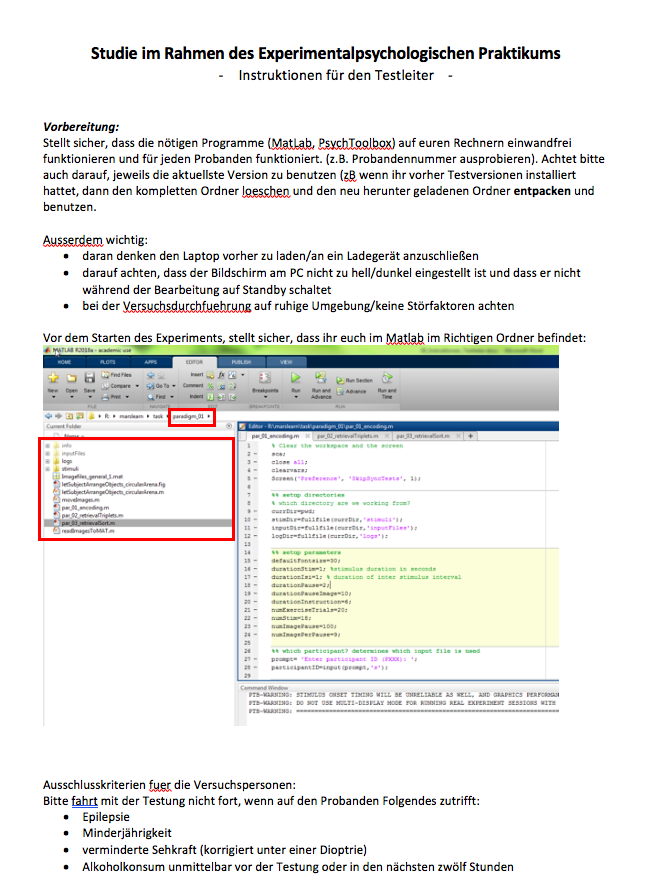
\includegraphics[width=105mm]{Bilder/Testleiter.png}
\end{figure}

\newpage

\section{Instruktion ProbandInnen}
\begin{figure}[h]
    \centering
    
\includegraphics[width=100mm]{Bilder/ProbVOR.png}
    \caption{Instruktion vor der Testung}
\end{figure}
\newpage

%\begin{figure}[h]
    %\centering
    %
\includegraphics[width=90mm]{Bilder/ProbT1.png}
    %\caption{Instruktion zum ersten Messzeitpunkt}
%\end{figure}

%\begin{figure}[h]
    %\centering
    %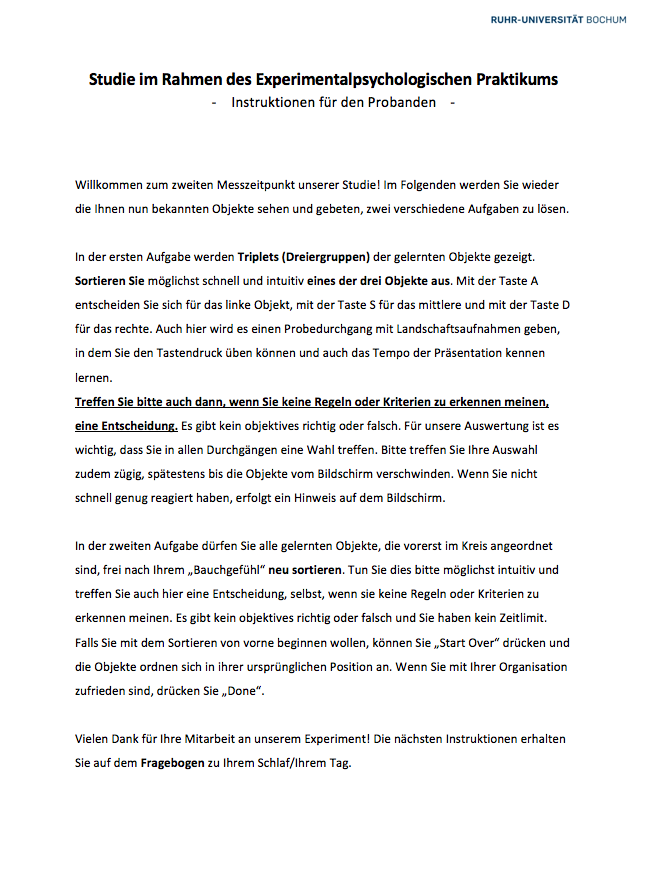
\includegraphics[width=85mm]{Bilder/ProbT2.png}
    %\caption{Instruktion zum zweiten Messzeitpunkt}
%\end{figure}

\begin{figure}[H]
  \centering
  \captionsetup[subfigure]{labelformat=empty}
  \setkeys{Gin}{width=66mm,keepaspectratio}%
  \vspace{0.5 cm}
  \subfloat[Instruktion Messzeitpunkt 1]{
\includegraphics{Bilder/ProbT1.png}} 
  \hspace{0.5cm}
  \subfloat[Instruktion Messzeitpunkt 2]{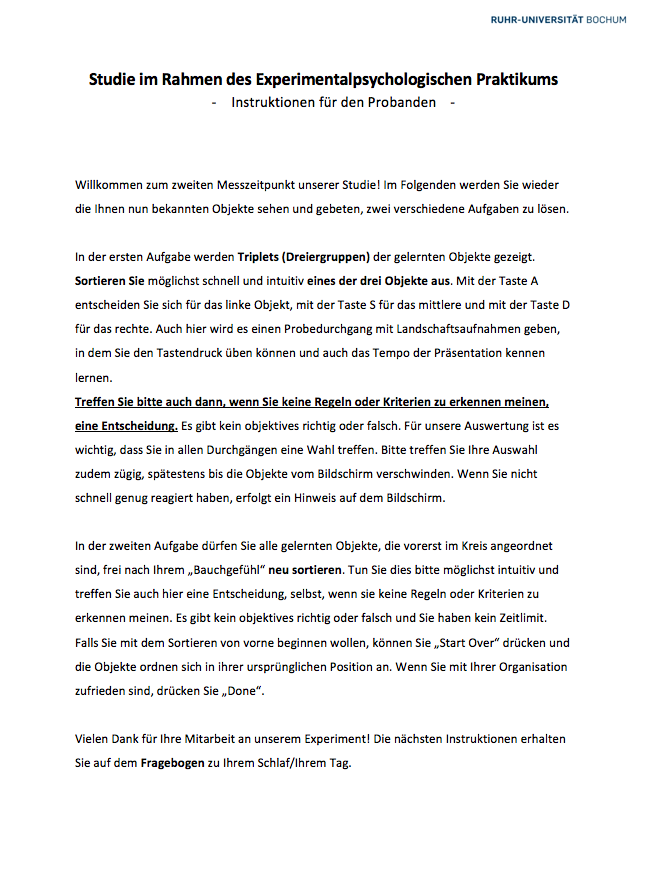
\includegraphics{Bilder/ProbT2.png}}
\end{figure}
\newpage

\section{Stimulus-Set}
\begin{figure}[H]
  \centering
  \captionsetup[subfigure]{labelformat=empty}
  \setkeys{Gin}{width=2.5in,height=2.5cm,keepaspectratio}%
  \subfloat[Obj. 1a]{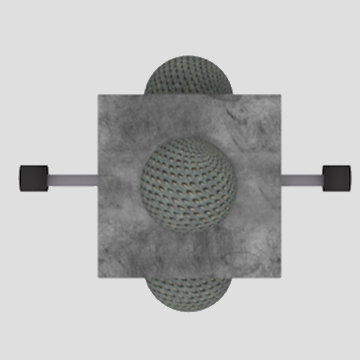
\includegraphics{Bilder/Objekt1A.png}}
  \hspace{0.5cm}
  \subfloat[Obj. 1b]{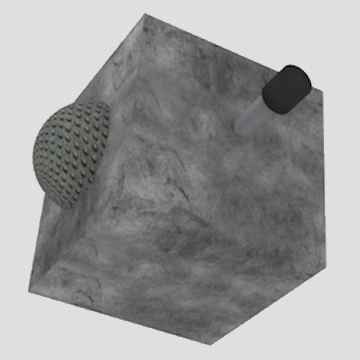
\includegraphics{Bilder/Objekt1B.png}} 
  \hspace{0.5cm}
  \subfloat[Obj. 2a]{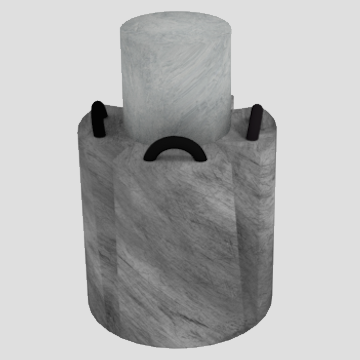
\includegraphics{Bilder/Objekt2A.png}}
  \hspace{0.5cm}
  \subfloat[Obj. 2b]{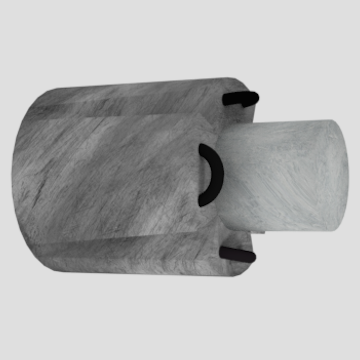
\includegraphics{Bilder/Objekt2B.png}} \\
  \subfloat[Obj. 3a]{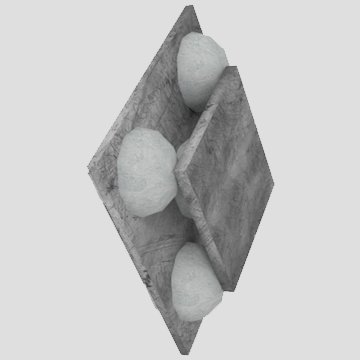
\includegraphics{Bilder/Objekt3A.png}}
  \hspace{0.5cm}
  \subfloat[Obj. 3b]{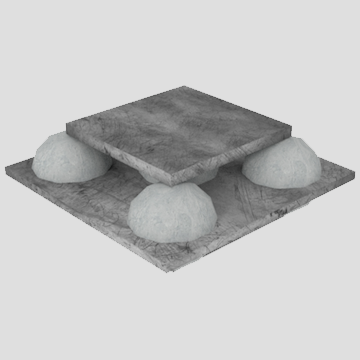
\includegraphics{Bilder/Objekt3B.png}}
  \hspace{0.5cm}
  \subfloat[Obj. 4a]{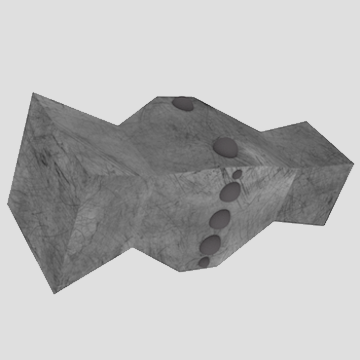
\includegraphics{Bilder/Objekt4A.png}}
  \hspace{0.5cm}
  \subfloat[Obj. 4b]{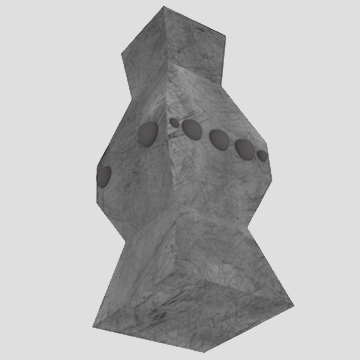
\includegraphics{Bilder/Objekt4B.png}}
  \caption{Note. a = originale Ausrichtung, b = rotiert}
\end{figure}

\begin{figure}[H]
  \ContinuedFloat\centering
  \captionsetup[subfigure]{labelformat=empty}
  \setkeys{Gin}{width=2.5in,height=2.5cm,keepaspectratio}%
  \subfloat[Obj. 5a]{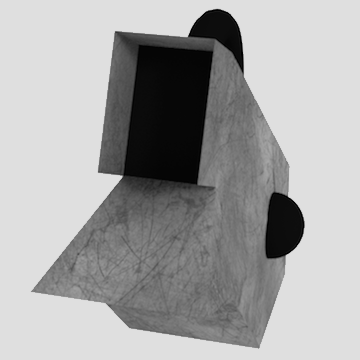
\includegraphics{Bilder/Objekt5A.png}}
  \hspace{0.5cm}
  \subfloat[Obj. 5b]{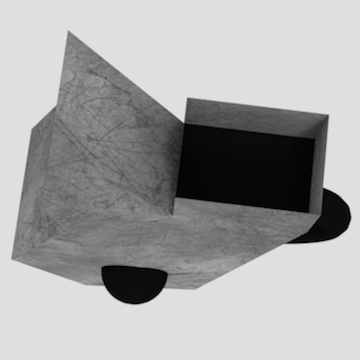
\includegraphics{Bilder/Objekt5B.png}}
  \hspace{0.5cm}
  \subfloat[Obj. 6a]{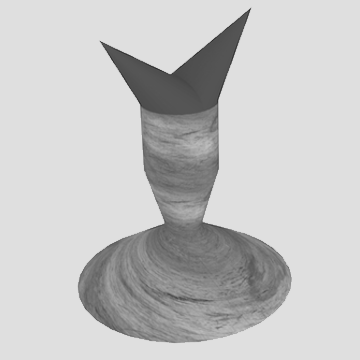
\includegraphics{Bilder/Objekt6A.png}}
  \hspace{0.5cm}
  \subfloat[Obj. 6b]{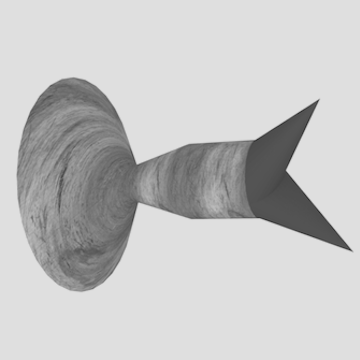
\includegraphics{Bilder/Objekt6B.png}}\\
  \subfloat[Obj. 7a]{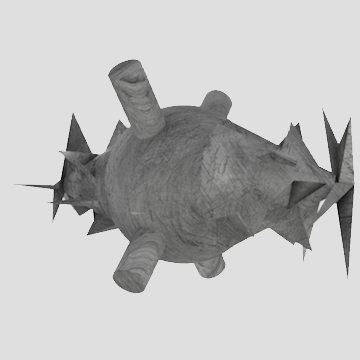
\includegraphics{Bilder/Objekt7A.png}}
  \hspace{0.5cm}
  \subfloat[Obj. 7b]{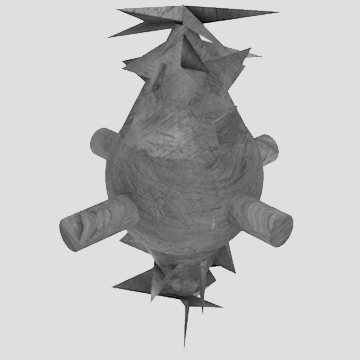
\includegraphics{Bilder/Objekt7B.png}}
  \hspace{0.5cm}
  \subfloat[Obj. 8a]{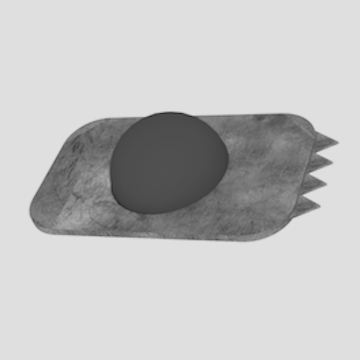
\includegraphics{Bilder/Objekt8A.png}}
  \hspace{0.5cm}
  \subfloat[Obj. 8b]{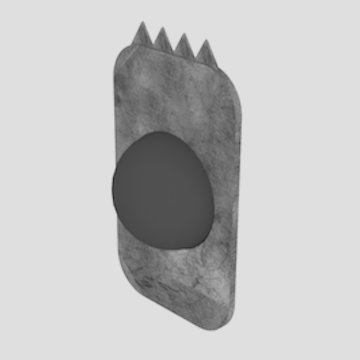
\includegraphics{Bilder/Objekt8B.png}}\\
  \subfloat[Obj. 9a]{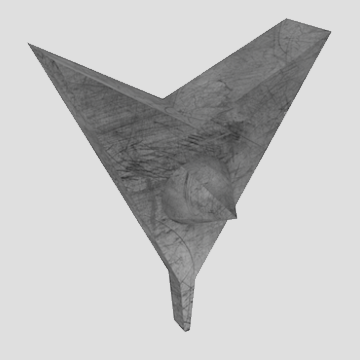
\includegraphics{Bilder/Objekt9A.png}}
  \hspace{0.5cm}
  \subfloat[Obj. 9b]{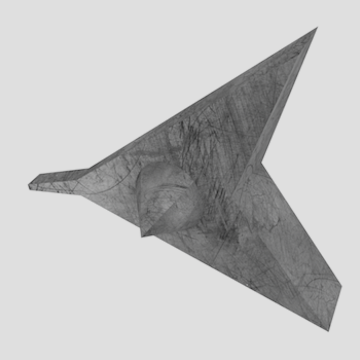
\includegraphics{Bilder/Objekt9B.png}}
  \hspace{0.5cm}
  \subfloat[Obj. 10a]{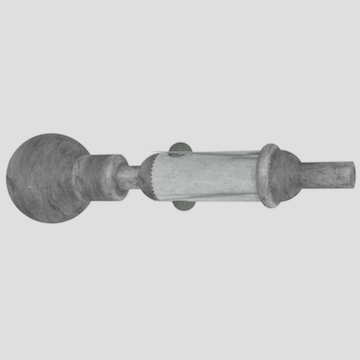
\includegraphics{Bilder/Objekt10A.png}}
  \hspace{0.5cm}
  \subfloat[Obj. 10b]{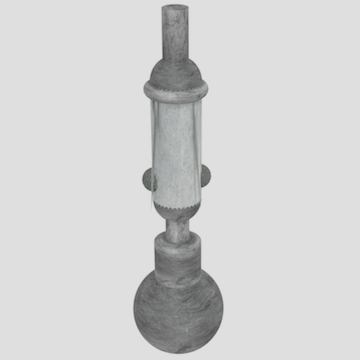
\includegraphics{Bilder/Objekt10B.png}}\\
   \subfloat[Obj. 11a]{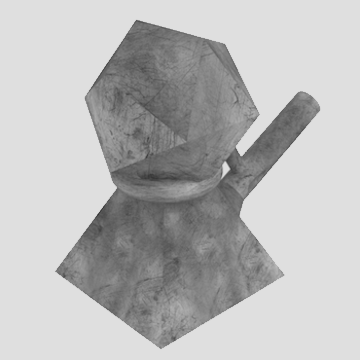
\includegraphics{Bilder/Objekt11A.png}}
  \hspace{0.5cm}
  \subfloat[Obj. 11b]{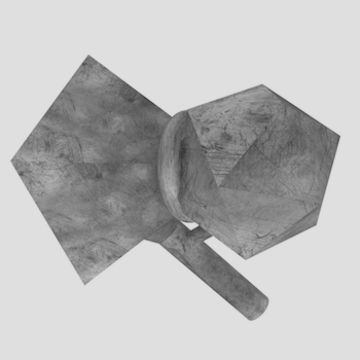
\includegraphics{Bilder/Objekt11B.png}}
  \hspace{0.5cm}
  \subfloat[Obj. 12a]{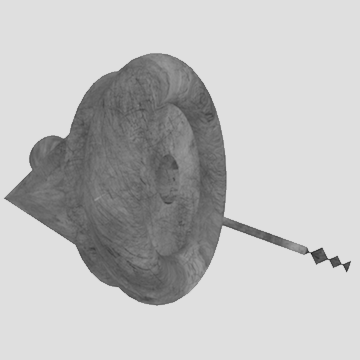
\includegraphics{Bilder/Objekt12A.png}}
  \hspace{0.5cm}
  \subfloat[Obj. 12b]{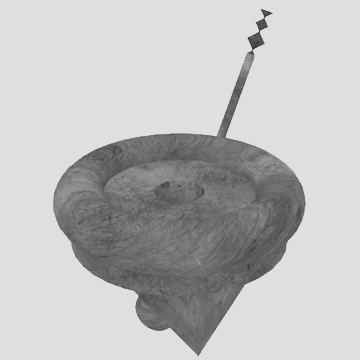
\includegraphics{Bilder/Objekt12B.png}}\\
   \subfloat[Obj. 13a]{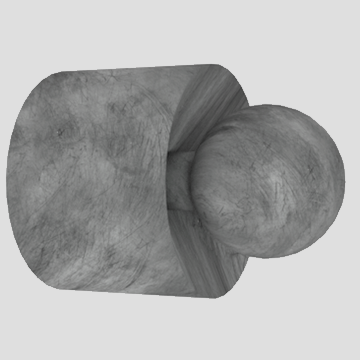
\includegraphics{Bilder/Objekt13A.png}}
  \hspace{0.5cm}
  \subfloat[Obj. 13b]{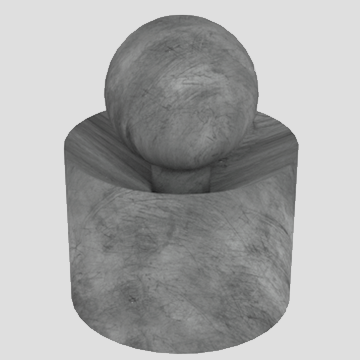
\includegraphics{Bilder/Objekt13B.png}}
  \hspace{0.5cm}
  \subfloat[Obj. 14a]{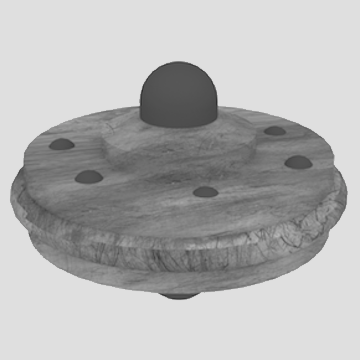
\includegraphics{Bilder/Objekt14A.png}}
  \hspace{0.5cm}
  \subfloat[Obj. 14b]{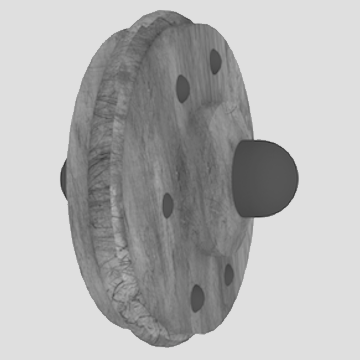
\includegraphics{Bilder/Objekt14B.png}}\\
  \end{figure}
  
  \begin{figure}[H]
  \ContinuedFloat\centering
  \captionsetup[subfigure]{labelformat=empty}
  \setkeys{Gin}{width=2.5in,height=2.5cm,keepaspectratio}%
   \subfloat[Obj. 15a]{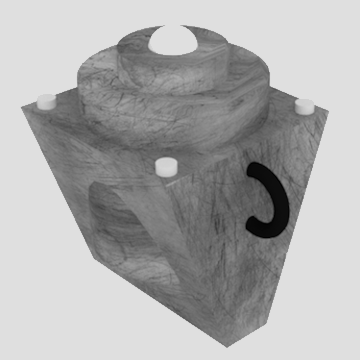
\includegraphics{Bilder/Objekt15A.png}}
  \hspace{0.5cm}
  \subfloat[Obj. 15b]{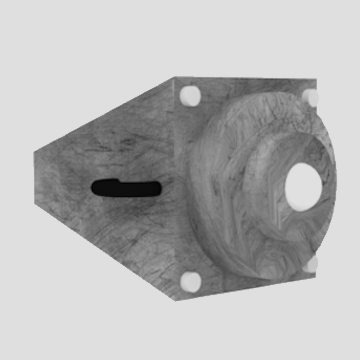
\includegraphics{Bilder/Objekt15B.png}}
  \hspace{0.5cm}
  \subfloat[Obj. 16a]{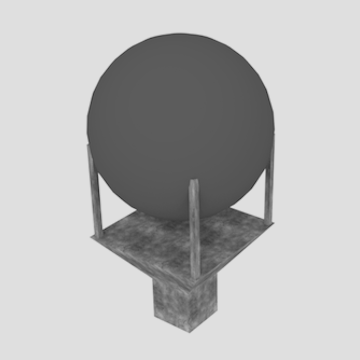
\includegraphics{Bilder/Objekt16A.png}}
  \hspace{0.5cm}
  \subfloat[Obj. 16b]{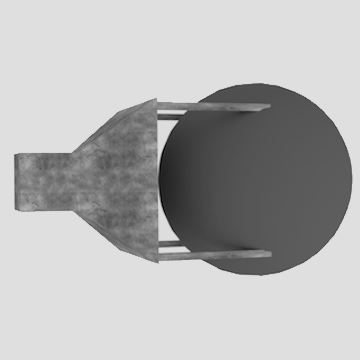
\includegraphics{Bilder/Objekt16B.png}}\\
   \subfloat[Obj. 17a]{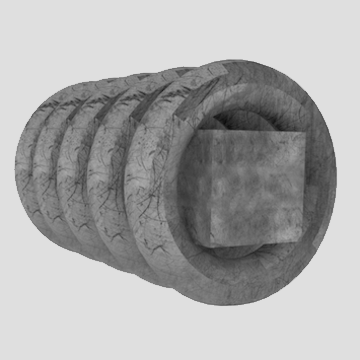
\includegraphics{Bilder/Objekt17A.png}}
  \hspace{0.5cm}
  \subfloat[Obj. 17b]{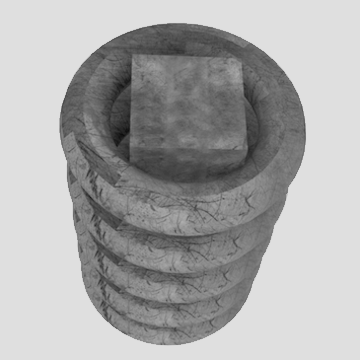
\includegraphics{Bilder/Objekt17B.png}}
  \hspace{0.5cm}
  \subfloat[Obj. 18a]{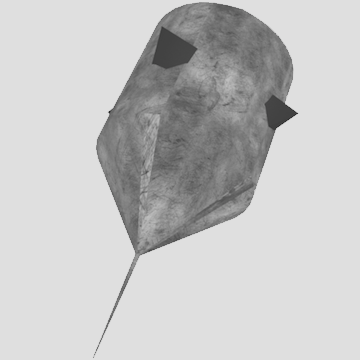
\includegraphics{Bilder/Objekt18A.png}}
  \hspace{0.5cm}
  \subfloat[Obj. 18b]{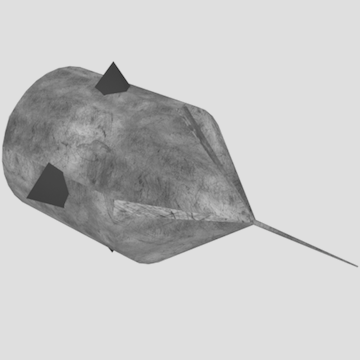
\includegraphics{Bilder/Objekt18B.png}}\\
  \caption{Note. a = originale Ausrichtung, b = rotiert}
\end{figure}
\newpage

\section{Triplet-Tabelle}
%\appendix

\begin{table}[h]
\centering
\captionsetup{justification=centering, margin = 1cm}
\begin{tabular}{l c c c c c c c c}
\hline
\textbf{Kategorie} & \multicolumn{3}{c}{\textbf{Community}} &  \multicolumn{3}{c}{\textbf{Distanz}} & \textbf{Anz. Trials} & \textbf{Vorh.}\\
& A & B & C & AB & BC & AC \\
\hline
1 & 1 & 1 & 1 & 1 & 1 & 3 & 18 & not B\\
2 & 1 & 1 & 1 & 1 & 2 & 3 & 12 & C\\
3 & 1 & 1 & 2 & 2 & 2 & 2 & 6 & C\\
4 & 1 & 1 & 2 & 1 & 2 & 1 & 12 & C\\
5 & 1 & 1 & 2 & 3 & 4 & 1 & 6 & not A\\
6 & 1 & 2 & 3 & 1 & 4 & 5 & 6 & C\\
7 & 1 & 2 & 3 & 4 & 4 & 4 & 18 & random\\
8 & 1 & 2 & 3 & 4 & 3 & 5 & 18 & A\\
\hline
\end{tabular}
\caption{Note. Anz. Trials = Anzahl der Durchgänge, Vorh. = Vorhersage, relevant für die Trefferquote}
\end{table}

\todo[inline]{BESCHREIBUNG DER TRIPLETS NOCH REIN? Und was ist mit den FRAGEBÖGEN?!?!}


%%%%%%%%%%%%%%%%%%%%%%%%%%%%%%%%%%

\newpage
\clearpage
%\phantomsection

\end{document}
